\msusection{Creating Graphs}\label{YC:sec:graphs}
\newcommand{\nitem}[1]{\item{\textbf{#1}}}
One of the main purposes of YCweather is to produce graphs, these graphs are meant to be customizable and easily exportable.  This section details the creation and manipulation available in YCweather created graphs.  Graphs are generated using the Data List window as demonstrated in the previous section.

\msusubsection{Dual-axis}
When creating a graph, the Data List window (Figure \ref{fig:datalist}) displays two tabs.  Data selected via the Primary and Secondary tabs graph along the left-side and right-side vertical axis, respectively.  For example, Figure \ref{fig:dualaxis} was created by selecting Air Temperature under the Primary tab and Incoming Short-wave under the Secondary Tab. The tick marks along the axes are setup to coincide, this sometimes results in illogical tick mark labels.  This problem may be corrected by editing the limits and step size, which is detailed in the following section.

\begin{figure}[ht!]\centering
	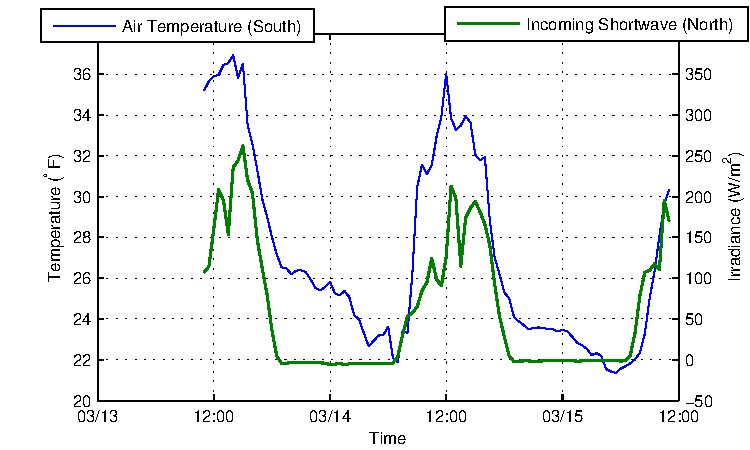
\includegraphics{\YCfiles figures/dualaxis.pdf}
	\caption{Example graph showing dual-axis capabilities.}
	\label{fig:dualaxis}
\end{figure}

\msusubsection{Editing Axis Limits and Step-size}\label{sec:editlimit}
In many cases, especially when creating graphs for dissemination, it is desirable to change the tick marks and limits on the graph.  YCweather provides this capability via two options: Limit Boxes and Step-size Boxes.  These options are available on the figure toolbar by the pairs of green arrows or by selecting the options from the corresponding axis menu (e.g., the X-axis menu).
\begin{itemize}
	\nitem{Limit Boxes:} This option creates two text box items near the extremes of the corresponding axis.  Simply change the limits to the desired value and press Enter.  If the box is empty the axis limits are automatically determined based on the data.
	\nitem{Step-size Boxes:} This toggle places a text box item near the lower axis limit.  This value dictates the step size between tick marks; leaving the value empty results in automatic tick placement.
\end{itemize}

\msusubsection{Exploring Data}\label{sec:exploredata}
The YCweather graphs allow the user to explore the data in various ways.

\begin{enumerate}
		\nitem{Limit/Step-size Boxes} allow for custom control of axis limits and tick marks, see Section \ref{sec:editlimit} for more details.
		\nitem{Zooming}: This option is toggled by selecting the magnifying glass icon on the figure toolbar. 
		\nitem{Data Cursor} allows the user to view the actual numbers associated with the graph by selecting a portion of the plotted line.  This option is available on the figure toolbar.
		\nitem{Zoom Slider} operates similar to the zooming feature but restricts the zoom to the associated axis and has a slider bar that controls the zooming from 100\% to 0.1\% of the data range.  The slider feature is available in the menus associated with each axis (e.g., X-Axis menu).
		\nitem{Line highlighting} is activated by left-clicking the mouse button on the desired line, this will make the line large and display the actual data points that make up the line.  The highlighting is removed by left-clicking the line a second time.
\end{enumerate}

\msusubsection{Context Menus}
The lines, labels, and legends on YCweather graphs each have menus associated that allow the user to manipulate the data.  The menus for these items are accessed by right-clicking on the object.

\begin{itemize}
	\nitem{Line Context Menu:}  By right clicking on any line the user has control over the appearance of the line for items such as the line thickness, style, color, or markers.  Additionally, a line may be deleted.
	\nitem{Label Context Menu:}  Each text item, such as the axis labels or annotations (see Section \ref{sec:axismenu}), allows for the user to edit the text, font, and location or delete the item. 
	\nitem{Legend Context Menu:}  The legend is also editable in its appearance including options for editing the color of the box or the width of the bounding box.  Also, when two legends are present. as in Figure \ref{fig:dualaxis}. they may be combined into a single legend by selecting the refresh option in this menu.  Then simply delete the unwanted legend box.
\end{itemize}
	
\msusubsection{Figure Menus}\label{sec:axismenu}
The axes menus available from graphs created with YCweather include the Options menu as well as a menu for each axis.  The Options menu provides generic functionality that applies to the entire figure whereas the axis specific menus only apply to that axis.

\msusubsubsection{File menu (default MATLAB menu)}
\begin{itemize}
	\nitem{New:} This option creates an empty figure, which is unaccessible with YCweather.
	\nitem{Open:} Allows the user to open figure files that were saved with the *.fig extension.
	\nitem{Close:} Closes the current figure.
	\nitem{Save:} Saves the figure by overwriting the current file if the figure has previously been saved, otherwise it envokes the Save as option.
	\nitem{Save as:} Allows the user to save the figure in a vareity of formats, including MATLAB *.fig format.
	\nitem{Export Setup:} Opens MATLAB's export user interface (see Section \ref{sec:exportfig}).
	\nitem{Print Preview:} Opens MATLAB's print setup user interface (see Section \ref{sec:exportfig}).
	\nitem{Print:} Sends the figure to the printer.
\end{itemize}

\msusubsubsection{Options menu}
\begin{itemize}
     \nitem{Add/Edit Labels:} Allows user to add and/or edit the axes labels, figure name, and figure title.
     \nitem{Interperter:} Allows user to change the typesetting format, \TeX\ and \LaTeX\ are usefull when equations and units are being displayed.
     \nitem{Edit Font:} Allows the user to change the font, style, and size for all text objects in the figure.
     \nitem{Axes Color:} Controls the background color of the figure.
     \nitem{Add Annotation:} Enables user to insert items such as text boxes and arrows.
     \nitem{Resize Figure:} Allows for editing the size of the figure, which is useful for exporting.
     \nitem{Tight Fit:} Moves the axis labels to the outer extent to minimize whitespace around the edges, this option is irreversible.
     \nitem{Export figure:} Allows the user to export the figure as an image file (see Section \ref{sec:exportfig}).
\end{itemize}

\msusubsubsection{X-,Y-, and Y2-Axis Menus}
\begin{itemize}
     \nitem{Ticks/Labels:} Allows for strict definition of the tick marks and labels used on the associated axis. 
     \nitem{Step Size Box:} Toggle for the step size controls (see Section \ref{sec:editlimit}).
     \nitem{Limit Boxes:} Toggle for the axis limit controls (see Section \ref{sec:editlimit}).
     \nitem{Zoom Slider:} Toggles the presence of the zoom slider (see Section \ref{sec:exploredata}).
     \nitem{Grid:} Toggles the major grid lines.
     \nitem{Minor Grid:} Toggles the minor grid lines.
     \nitem{Minor Ticks:} Toggles the axis tick marks.
     \nitem{Reversed:} Toggles the orientation of the tick marks and labels along the axis.
	 \nitem{Add/Edit Legend:} Allows the user to add or edit the legend entries.
\end{itemize}

\msusubsection{Exporting Figures}\label{sec:exportfig}
YCweather allows the user to output the graphs in a variety of formats.  For those familiar with MATLAB, it is possible save the figure as a *.fig file.  The exporting/saving is accomplished in two ways.  First, to simply create an image exactly as the figure appears, select Export Figure from the Options Menu or press the associated Toolbar button (see Section \ref{sec:axismenu}).  This option will output the figure exactly as it appears, so it is imperative to setup the figure precisely as needed.  The size of the exported figure can be specified by editing the dimensions via the Resize Figure option in the Options Menu.

The second option for saving/exporting figures is accomplished using the File Menu (Section \ref{sec:axismenu}), this menu is the default MATLAB figure menu; thus, for users unfamiliar with MATLAB these options may be difficult to use.  This menu provides two options: one for printing the image that uses the Print Preview and Print menu items and an Export Setup option for saving the figure as an image.  Both, the Print Preview and Export Setup open user interfaces with a variety of options, details for using these items may be found in the online MATLAB help file: \href{http://www.mathworks.com/access/helpdesk/help/techdoc/index.html}{\nolinkurl{http://www.mathworks.com/access/helpdesk/help/techdoc/index.html}} (in the contents select ``Graphics''; ``Printing and Exporting''; ``How to Print or Export'').

